\subsection{Fashion-MNIST: khai thác mẫu trực quan}

\subsubsection{Bài toán và tập dữ liệu}

Fashion-MNIST cho phép khảo sát cách áp dụng Eclat cho ảnh. Nhóm
gán mã cho các vùng ảnh có đặc trưng tương tự. Mỗi mã được gọi là
một từ thị giác (\textit{visual word}). Giao dịch của một ảnh gồm
các mã có mặt trong ảnh đó. Tập mục phổ biến vì vậy là tổ hợp mã
thường xuất hiện cùng nhau.

Tập dữ liệu gồm 70.000 ảnh xám $28\times28$ pixel thuộc mười lớp,
với 6.000 ảnh huấn luyện và 1.000 ảnh kiểm thử cho mỗi lớp~\cite{Xiao2017}.
Kích thước đồng nhất cho phép dùng chung một lưới chia vùng. Số ảnh
bằng nhau giữa các lớp giúp so sánh tỷ lệ xuất hiện của mẫu. Thí nghiệm
dùng cả hai tập gốc để mô tả các mẫu trên toàn bộ dữ liệu.

\subsubsection{Tạo giao dịch bằng BoVW nhị phân}

Hình~\ref{fig:fashion_tc_pipeline} tóm tắt các bước chuyển ảnh Fashion-MNIST thành cơ sở dữ liệu giao dịch bằng BoVW nhị phân.

\begin{figure*}[!tbp]
    \centering
    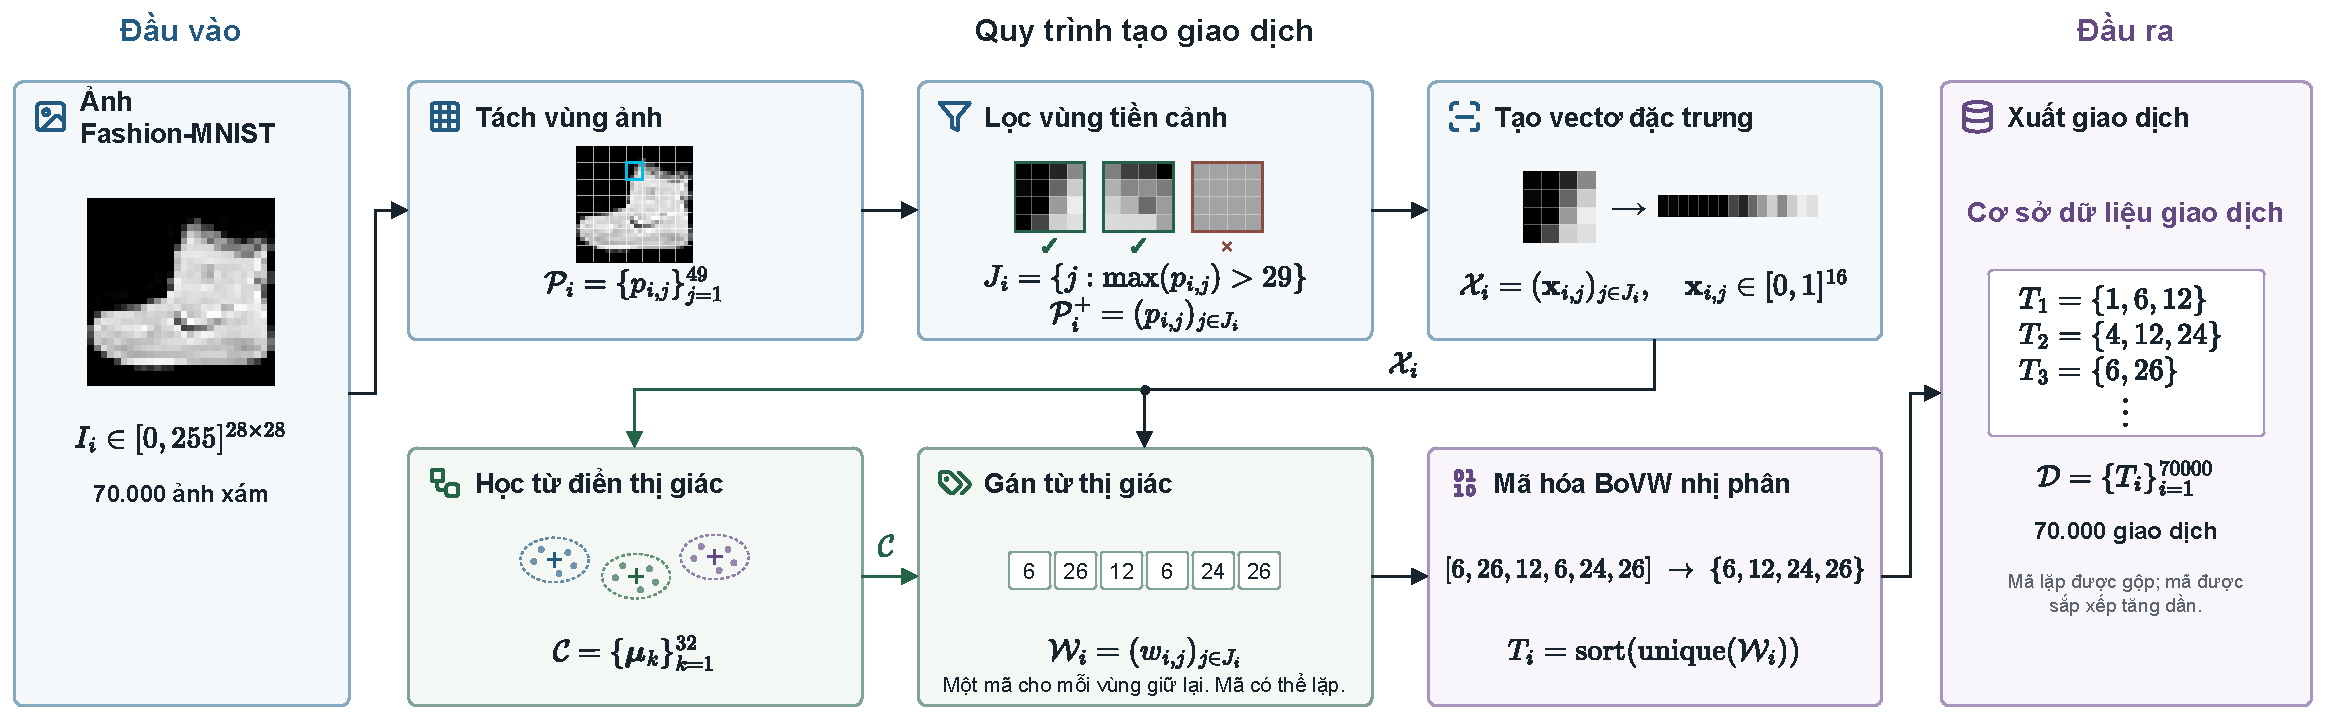
\includegraphics[width=\textwidth]{figures/diagram/TC_pipeline.pdf}
    \caption{Quy trình tạo giao dịch từ ảnh Fashion-MNIST. Nhóm học một từ điển chung từ các vùng giữ lại trên toàn bộ 70.000 ảnh rồi dùng từ điển đó để gán mã cho từng vùng. Các mã và giao dịch trong hình dùng để minh họa.}
    \label{fig:fashion_tc_pipeline}
\end{figure*}

Nhóm dùng túi từ thị giác (\textit{bag of visual words}, BoVW)~\cite{Sivic03}
để biểu diễn mỗi ảnh bằng các vùng ảnh nhỏ (\textit{patch}).
Trong khảo sát tiền xử lý, ở mức loại khoảng 39,3\% số vùng,
vùng kích thước $4\times4$ pixel làm mất 5,92\% tổng độ lớn gradient,
so với 14,00\% khi dùng vùng $7\times7$ pixel. Nhóm chọn kích thước
$4\times4$ pixel để giữ được nhiều biến thiên mức xám cục bộ hơn.

Mỗi ảnh $28\times28$ pixel được chia thành lưới $7\times7$ gồm
49 vùng không chồng lấn, mỗi vùng có kích thước $4\times4$ pixel.
Nhóm giữ vùng có ít nhất một pixel với mức xám lớn hơn 29. Giá trị 29 là phân vị
thứ 10 của các pixel khác 0. Quy tắc này loại 37,50\% số vùng,
làm mất 4,41\% tổng độ lớn gradient và vẫn giữ được vùng ảnh ở
cả 70.000 ảnh. Mỗi vùng được biểu diễn bằng vectơ đặc trưng
(\textit{descriptor}) gồm 16 giá trị mức xám, chuẩn hóa về $[0,1]$.

K-means~\cite{lloyd} gom các vectơ thành 32 cụm. Các tâm cụm
$\mathcal{C}=\{\boldsymbol{\mu}_k\}_{k=1}^{32}$ tạo thành từ điển
thị giác. Mỗi vectơ $\mathbf{x}_{i,j}$ của vùng $j$ trong ảnh $i$
nhận mã của tâm gần nhất
\begin{equation}
 w_{i,j}=\arg\min_{1\leq k\leq32}
          \|\mathbf{x}_{i,j}-\boldsymbol{\mu}_k\|_2^2.
\end{equation}
Bảng~\ref{tab:kmeans_configuration} trình bày cấu hình đã dùng.
Kết quả khảo sát số cụm được trình bày ở Phụ lục~\ref{sec:fashion-reproduction}.

\begin{table}[!t]
    \centering
        \caption{Cấu hình K-means trong thí nghiệm Fashion-MNIST}
    \label{tab:kmeans_configuration}
    \footnotesize
    \setlength{\tabcolsep}{3pt}
    \begin{tabular}{@{}p{0.40\columnwidth} p{0.55\columnwidth}@{}}
        \hline
        \textbf{Tham số} & \textbf{Giá trị} \\
        \hline
        Phương pháp & K-means toàn bộ, khởi tạo K-means++~\cite{kmpp} \\
        Dữ liệu phân cụm & 2.143.746 vectơ từ 70.000 ảnh \\
        Vectơ đặc trưng & 16 giá trị pixel xám đã chuẩn hóa \\
        Số cụm ($K$), seed & 32, 123 \\
        Giới hạn lặp, dung sai & 400, $10^{-4}$ \\
        \hline
    \end{tabular}
\end{table}

Với ảnh $I_i$, gọi $J_i$ là tập chỉ số các vùng được giữ lại và
$\mathcal{W}_i=(w_{i,j})_{j\in J_i}$ là dãy mã của các vùng đó.
BoVW nhị phân tạo giao dịch
$T_i=\operatorname{sort}(\operatorname{unique}(\mathcal{W}_i))$.
Mỗi mã được ghi một lần và các mã được sắp tăng dần. Tọa độ vùng
được lưu riêng để truy vết. Sau bước này, cả 70.000 giao dịch đều
có ít nhất một mã, với độ dài trung bình khoảng 12,23 mã.

Khảo sát năm kích thước từ điển với ba seed chọn $K=32$ làm cấu hình
cơ sở: ở ngưỡng hỗ trợ 3\%, số cặp phổ biến trung bình là 487,3,
so với 120 tại $K=16$ và 1.451,3 tại $K=64$; độ dài giao dịch trung
bình tại $K=32$ là 12,26 mã, thấp hơn mức 15,04 mã tại $K=64$.
BoVW nhị phân được giữ làm biểu diễn chính vì mỗi giao dịch chỉ ghi
nhận các mã khác nhau cùng xuất hiện, không gắn chúng với vị trí cố
định. Các biểu diễn theo vùng và dải được dùng để đối chiếu ảnh hưởng
của vị trí. Độ méo tiếp tục giảm khi tăng $K$, nên $K=32$ là lựa chọn
thực dụng theo độ gọn và khối lượng mẫu cần rà soát, không phải mức
tối ưu đã được chứng minh. Bảng khảo sát nhiều seed được trình bày ở
Phụ lục~\ref{sec:fashion-reproduction}.

\subsubsection{Thiết kế thực nghiệm khai thác}
Nhóm dùng Eclat với Set và BitVector trên cùng bộ giao dịch BoVW
nhị phân, ở sáu ngưỡng hỗ trợ từ 80\% đến 5\%. Dải ngưỡng cho
phép quan sát từ những tổ hợp có mặt trong phần lớn ảnh đến
những tổ hợp ít gặp hơn nhưng vẫn xuất hiện trong ít nhất
3.500 ảnh. Bảng~\ref{tab:eclat_backend_comparison} ghi số hỗ trợ
tối thiểu tương ứng với từng ngưỡng.

Với mỗi ngưỡng, nhóm đối chiếu từng tập mục và số hỗ trợ giữa
hai phiên bản. Thời gian được đo trong tiến trình Julia riêng.
Mỗi cấu hình được đo một lần, từ đọc giao dịch đến ghi kết quả,
không có lượt làm nóng.

\subsubsection{Kết quả K-means và khai thác tập mục phổ biến}
\label{subsec:fashion_fim_results}

K-means hội tụ sau 220 vòng và mất 137,47 giây. Cả 32 cụm đều
có vectơ được gán, với 11,75\% số vectơ thuộc cụm lớn nhất.
Khoảng cách bình phương trung bình từ vectơ đến tâm được gán
là 0,351112. Entropy chuẩn hóa đạt 0,9265 trên thang từ 0 đến 1,
cho thấy các vectơ được phân bố qua nhiều cụm.

Hai phiên bản trả về cùng các tập mục và cùng số hỗ trợ ở cả
sáu ngưỡng. Khi hạ ngưỡng, mọi tập đã tìm được ở ngưỡng cao hơn
đều vẫn xuất hiện trong kết quả (Bảng~\ref{tab:eclat_backend_comparison}).

\begin{table}[!t]
    \centering
    \caption{Số tập mục phổ biến theo ngưỡng hỗ trợ}
    \label{tab:eclat_backend_comparison}
    \footnotesize
    \setlength{\tabcolsep}{4pt}
    \begin{tabular}{@{}c r r r c@{}}
        \toprule
        \textbf{Ngưỡng} & \textbf{Số hỗ trợ tối thiểu} &
        \textbf{Set} & \textbf{BitVector} & \textbf{Giống nhau} \\
        \midrule
        80\% & 56.000 & 0 & 0 & Có \\
        60\% & 42.000 & 1 & 1 & Có \\
        40\% & 28.000 & 11 & 11 & Có \\
        20\% & 14.000 & 145 & 145 & Có \\
        10\% & 7.000 & 1.098 & 1.098 & Có \\
         5\% & 3.500 & 6.185 & 6.185 & Có \\
        \bottomrule
    \end{tabular}
\end{table}

Ở ngưỡng 5\%, Eclat tìm được 6.185 tập phổ biến, trong đó các
tập có ba hoặc bốn mã chiếm 83,25\%. Phụ lục~\ref{sec:fashion-reproduction}
trình bày phân bố theo độ dài. Ở ngưỡng này, Set mất 20,94 giây
và BitVector mất 8,73 giây. Tại 40\%, Set lại nhanh hơn một chút
(Hình~\ref{fig:eclat_performance}). Các chênh lệch chỉ mô tả
một lượt chạy ở mỗi ngưỡng.

\begin{figure}[!t]
    \centering
    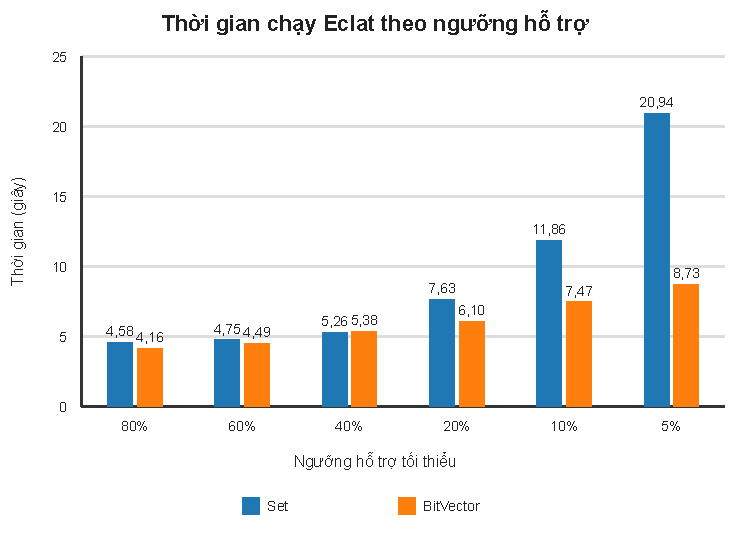
\includegraphics[width=\columnwidth]{figures/notebook3/eclat_performance.pdf}
    \caption{Thời gian chạy một lượt theo ngưỡng hỗ trợ. Nhãn TID-set (Set) chỉ phiên bản dùng cấu trúc Set.}
    \label{fig:eclat_performance}
\end{figure}

\subsubsection{Truy vết một mẫu thị giác}
\label{subsec:visual_pattern_interpretation}

Mẫu $\{6,12\}$ là tập nhiều mã có độ hỗ trợ cao nhất trong
kết quả ở ngưỡng 5\%. Mẫu có mặt trong 29.223 ảnh, tương ứng
41,75\% toàn bộ dữ liệu. Phép đếm trực tiếp trên các giao dịch
cho cùng kết quả với Eclat.

Hình~\ref{fig:current_pattern_6_12} cho thấy hai vùng được
gán mã 6 và 12 trong một ảnh, bên cạnh hai tâm cụm tương ứng.
BoVW nhị phân ghi nhận sự có mặt của hai mã ở bất kỳ vị trí nào.
Các mã 6 và 12 được xác định theo từ điển của thí nghiệm.

\begin{figure*}[!tbp]
    \centering
    \begin{tabular}{ccccc}
        
\includegraphics[width=0.17\textwidth]{figures/current_pattern/supporting_image.png} &
        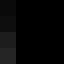
\includegraphics[width=0.17\textwidth]{figures/current_pattern/word_6_actual.png} &
        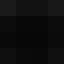
\includegraphics[width=0.17\textwidth]{figures/current_pattern/word_6_centroid.png} &
        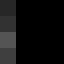
\includegraphics[width=0.17\textwidth]{figures/current_pattern/word_12_actual.png} &
        
\includegraphics[width=0.17\textwidth]{figures/current_pattern/word_12_centroid.png} \\
        Ảnh minh họa & Vùng mã 6 & Tâm mã 6 & Vùng mã 12 & Tâm mã 12
    \end{tabular}
    \caption{Ảnh và các vùng được truy vết cho mẫu $\{6,12\}$. Hai tâm cụm là các vectơ mức xám hiển thị dưới dạng vùng $4\times4$.}
    \label{fig:current_pattern_6_12}
\end{figure*}

\subsubsection{Phân bố mẫu theo lớp}
\label{subsec:fim_class_applications}

Gọi $P(X)$ là tỷ lệ ảnh chứa mẫu $X$ trên toàn bộ dữ liệu và
$P(X\mid c)$ là tỷ lệ ảnh chứa mẫu trong lớp $c$. Hai tỷ lệ này
cho phép tính hệ số làm giàu (\textit{enrichment})
\begin{equation}
    E(X,c)=\frac{P(X\mid c)}{P(X)}.
    \label{eq:fim_F_class_enrichment}
\end{equation}
Giá trị lớn hơn 1 cho biết tỷ lệ ảnh chứa mẫu trong lớp cao hơn tỷ lệ trên toàn bộ ảnh. Bảng~\ref{tab:pattern_class_distribution} ghi kết quả cho mẫu $\{6,12\}$.

\begin{table}[!t]
    \centering
    \caption{Phân bố mẫu $\{6,12\}$ theo lớp}
    \label{tab:pattern_class_distribution}
    \scriptsize
    \setlength{\tabcolsep}{2pt}
    \begin{tabular}{@{}l r r r@{}}
        \toprule
        \textbf{Lớp} & \textbf{Ảnh chứa mẫu} & \textbf{Tỷ lệ trong lớp} & \textbf{Hệ số làm giàu} \\
        \midrule
        T-shirt/top & 4.354 & 62,20\% & 1,490 \\
        Trouser & 1.263 & 18,04\% & 0,432 \\
        Pullover & 3.528 & 50,40\% & 1,207 \\
        Dress & 3.144 & 44,91\% & 1,076 \\
        Coat & 3.593 & 51,33\% & 1,230 \\
        Sandal & 3.360 & 48,00\% & 1,150 \\
        Shirt & 4.323 & 61,76\% & 1,479 \\
        Sneaker & 1.383 & 19,76\% & 0,473 \\
        Bag & 2.927 & 41,81\% & 1,002 \\
        Ankle boot & 1.348 & 19,26\% & 0,461 \\
        \bottomrule
    \end{tabular}
\end{table}

Mẫu xuất hiện ở cả mười lớp. Tỷ lệ dao động từ 18,04\% ở Trouser đến 62,20\% ở T-shirt/top. Chênh lệch này cho thấy cùng một mẫu có thể phổ biến hơn ở một số lớp dù xuất hiện rộng trong toàn bộ dữ liệu.

Nhãn lớp chỉ được dùng sau bước khai thác để tính các tỷ lệ.
Vì từ điển thị giác và các tập mục đều được xây dựng từ cả hai
tập ảnh gốc, các tỷ lệ này mô tả chính bộ dữ liệu đã khai thác.

\subsubsection{Mức độ làm giàu theo ngưỡng hỗ trợ}

Với mỗi tập mục $X$, đặt $E_{\max}(X)=\max_c E(X,c)$, tức hệ số làm giàu lớn nhất trong mười lớp. Bảng~\ref{tab:fashion_enrichment_thresholds} cho thấy cả trung vị $E_{\max}$ lẫn tỷ lệ tập mục có $E_{\max}\geq2$ tăng khi hạ ngưỡng hỗ trợ. Tại 5\%, 4.180 trong 6.185 tập mục (67,58\%) xuất hiện trong ít nhất một lớp với tỷ lệ gấp đôi tỷ lệ chung trở lên. Ở các ngưỡng từ 40\%, không có tập nào đạt mức này. Mức làm giàu còn phụ thuộc vào độ phổ biến chung của mẫu. Ví dụ, mẫu đã có mặt trong 60\% toàn bộ ảnh chỉ có thể đạt hệ số tối đa khoảng 1,67, kể cả khi xuất hiện trong mọi ảnh của một lớp.

\begin{table}[!t]
    \centering
    \caption{Hệ số làm giàu lớn nhất theo ngưỡng hỗ trợ}
    \label{tab:fashion_enrichment_thresholds}
    \scriptsize
    \setlength{\tabcolsep}{3pt}
    \begin{tabular}{@{}c r r r r@{}}
        \toprule
        \textbf{Ngưỡng} & \textbf{Số tập mục} & \textbf{Trung vị $E_{\max}$} &
        \textbf{$E_{\max}\geq2$} & \textbf{Tỷ lệ} \\
        \midrule
        80\% & 0 & -- & 0 & -- \\
        60\% & 1 & 1,294 & 0 & 0\% \\
        40\% & 11 & 1,490 & 0 & 0\% \\
        20\% & 145 & 1,735 & 26 & 17,93\% \\
        10\% & 1.098 & 1,998 & 543 & 49,45\% \\
         5\% & 6.185 & 2,225 & 4.180 & 67,58\% \\
        \bottomrule
    \end{tabular}
\end{table}

Hình~\ref{fig:fashion_enrichment_summary} cho thấy phân bố hệ số lớn nhất theo ngưỡng và số mẫu có hệ số từ 2 trở lên ở từng lớp. Trong khi biểu đồ (b) đếm mẫu riêng theo lớp, $E_{\max}$ chỉ lấy lớp có tỷ lệ tương đối cao nhất để mô tả mức tập trung của từng mẫu.

\begin{figure*}[!tbp]
    \centering
    \begin{minipage}[t]{0.48\textwidth}
        \centering
        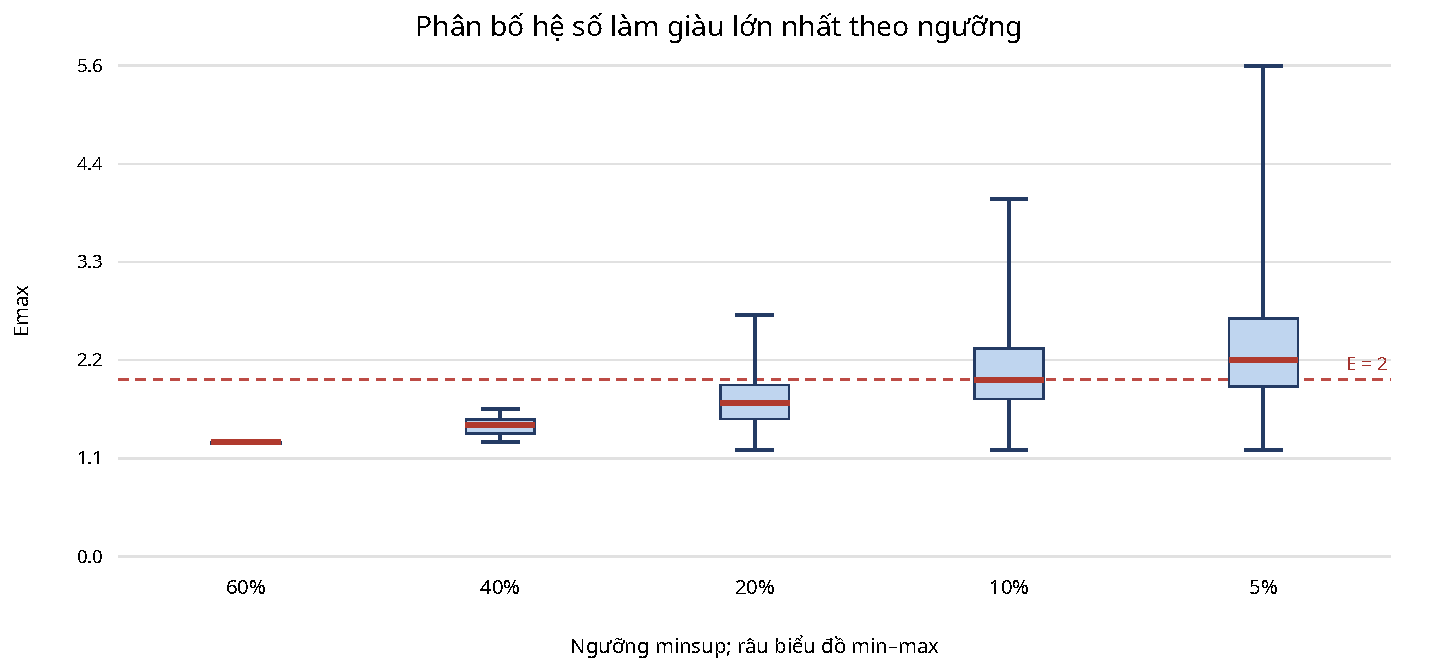
\includegraphics[width=\linewidth]{figures/notebook3/enrichment_by_threshold.pdf}
        \\
        \small (a) Phân bố $E_{\max}$ theo ngưỡng hỗ trợ.
    \end{minipage}\hfill
    \begin{minipage}[t]{0.48\textwidth}
        \centering
        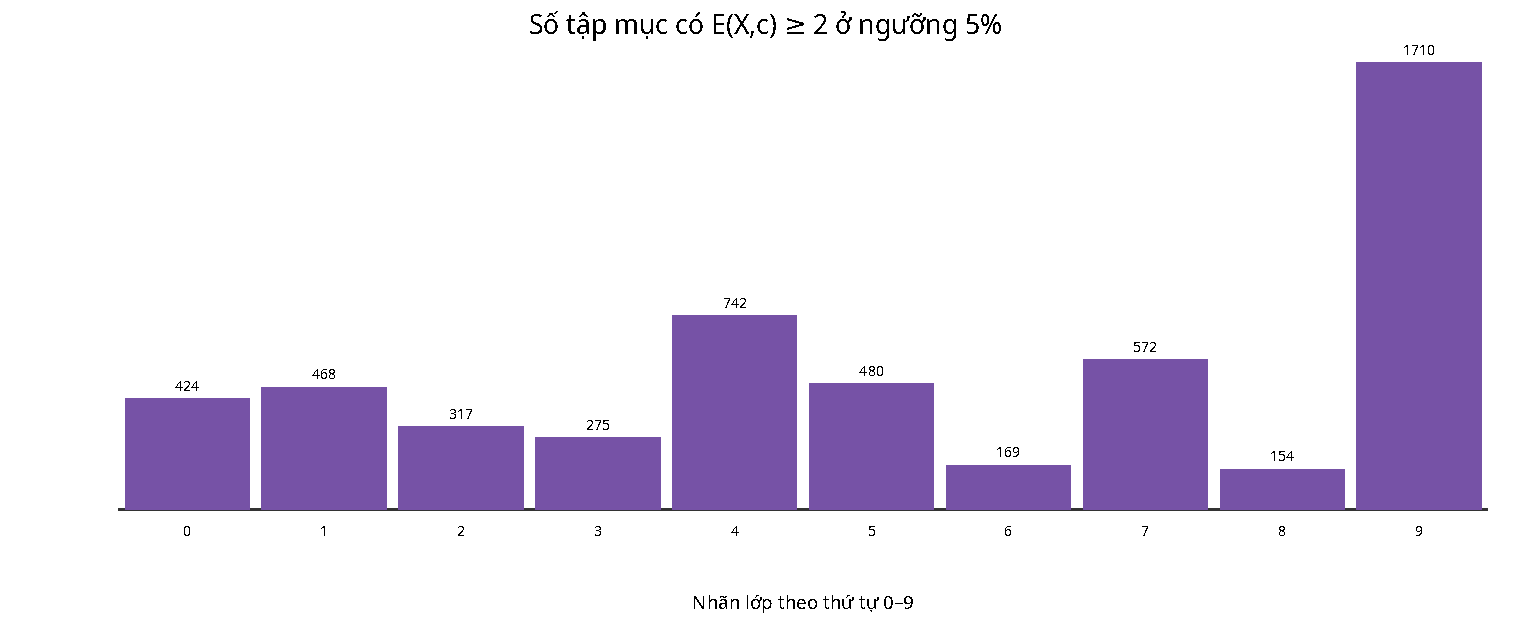
\includegraphics[width=\linewidth]{figures/notebook3/patterns_enriched_by_class.pdf}
        \\
        \small (b) Số tập mục có $E(X,c)\geq2$ theo lớp.
    \end{minipage}
    \caption{Mức độ làm giàu của các tập mục khai thác được. Các thanh dọc ở biểu đồ (a) biểu thị khoảng giá trị nhỏ nhất đến lớn nhất. Biểu đồ (b) đếm riêng theo từng lớp, nên một tập mục có thể xuất hiện trong nhiều cột.}
    \label{fig:fashion_enrichment_summary}
\end{figure*}

\subsubsection{Các mẫu nhiều mã nổi bật trong từng lớp}

Để xem tổ hợp từ thị giác nào gắn với từng lớp, nhóm chọn cho mỗi lớp một tập nhiều mã có $E(X,c)$ cao nhất trong số các tập mà ít nhất 10\% ảnh của lớp chứa tập đó. Hình~\ref{fig:fashion_class_pattern_heatmap} biểu diễn tỷ lệ chứa từng mẫu trên cả mười lớp. Ví dụ, mẫu $\{13,14,26,29\}$ có mặt trong 31,11\% ảnh Trouser và hệ số làm giàu 5,553; mẫu $\{3,10,15,22\}$ có mặt trong 25,91\% ảnh Ankle boot và hệ số 5,156.

\begin{figure*}[!tbp]
    \centering
    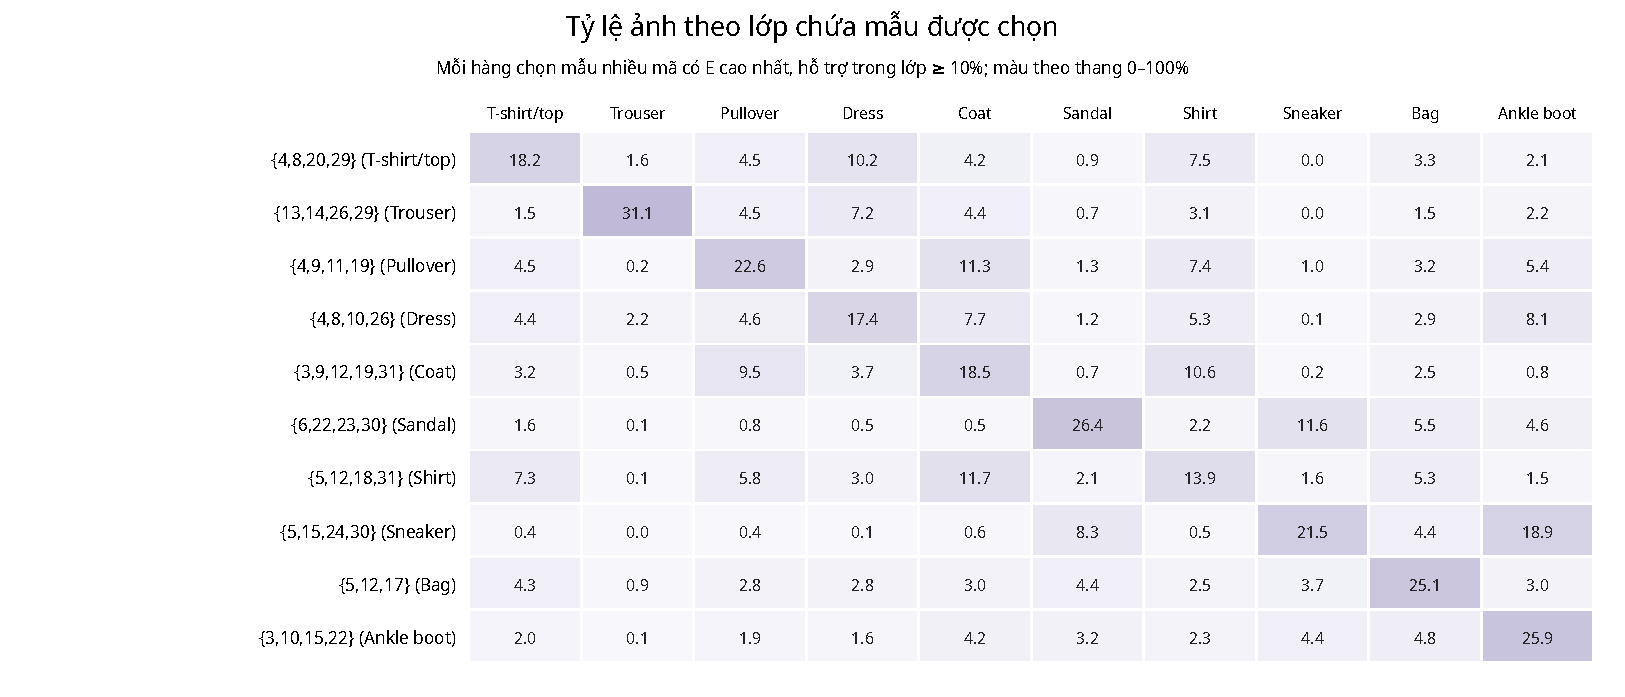
\includegraphics[width=0.98\textwidth]{figures/notebook3/class_pattern_heatmap.pdf}
    \caption{Tỷ lệ ảnh trong mỗi lớp chứa mẫu nhiều mã được chọn cho hàng đó. Mẫu của từng hàng được chọn theo hệ số làm giàu cao nhất, với điều kiện tỷ lệ hỗ trợ trong lớp đạt ít nhất 10\%.}
    \label{fig:fashion_class_pattern_heatmap}
\end{figure*}

Các ô ngoài đường chéo cho thấy mẫu được chọn ở một lớp cũng có thể xuất hiện ở lớp khác. Hình vì vậy giúp xác định mẫu nào đáng khảo sát tiếp. Giá trị dự đoán cần được đánh giá trên dữ liệu độc lập với bước chọn mẫu.

\subsubsection{Hướng ứng dụng và phát triển các mô hình khác}

Các tập mục thường gặp hơn ở một lớp là những đặc trưng ứng viên
cho mô hình phân loại. Có thể dùng các mẫu này để giải thích ảnh
chứa tổ hợp mã nào hoặc để truy vấn những ảnh có chung tổ hợp.

Với $m$ tập mục đã chọn $P_1,\ldots,P_m$, vectơ đặc trưng của ảnh $I_i$ là $\boldsymbol{\phi}(I_i)=(\phi_1(I_i),\ldots,\phi_m(I_i))$. Mỗi thành phần cho biết giao dịch $T_i$ có chứa tập mục tương ứng hay không:
\begin{equation}
    \phi_j(I_i)=\mathbf{1}\!\left[P_j\subseteq T_i\right],
    \qquad j=1,\ldots,m.
    \label{eq:fim_pattern_features}
\end{equation}
Nhóm có thể so sánh ba biểu diễn trên cùng cách chia dữ liệu:
BoVW nhị phân, vectơ chỉ báo tập mục và biểu diễn có xét vị trí.
Với mỗi biểu diễn, dùng cùng nhóm bộ phân loại, chẳng hạn hồi quy
logistic, SVM tuyến tính và cây quyết định. So sánh các giá trị của
số cụm, ngưỡng hỗ trợ, cấu hình không gian và tham số mô hình
theo cùng quy trình chọn tham số.

Đề xuất dùng kiểm định chéo phân tầng năm phần
(\textit{stratified five-fold cross-validation}) trên 60.000 ảnh
huấn luyện. Mỗi lượt học lại từ điển, khai thác và chọn mẫu, rồi
huấn luyện mô hình chỉ trên bốn phần. Phần còn lại dùng để đánh
giá cấu hình. Có thể báo cáo trung bình và độ lệch chuẩn của độ
chính xác và F1 vĩ mô qua năm lượt, kèm ma trận nhầm lẫn để xem những lớp dễ bị nhầm với nhau.

Sau khi chọn cấu hình, huấn luyện lại trên toàn bộ 60.000 ảnh
và đánh giá một lần trên 10.000 ảnh kiểm thử giữ riêng. Kết quả
so với BoVW nhị phân trên tập này sẽ cho biết đặc trưng tập mục
hoặc thông tin vị trí có cải thiện khả năng dự đoán hay không.
